\documentclass[10pt,letterpaper]{article}

\usepackage{cogsci}
\usepackage{pslatex}
\usepackage[nodoi]{apacite}
\usepackage{graphicx}
\usepackage[american]{babel}
\usepackage{amsmath}
\usepackage[section]{placeins}
\usepackage{enumitem}

\title{Children's Online Processing of Ad-Hoc Implicatures}
 
\author{{\large \bf Erica J. Yoon} \\
  \texttt{ejyoon@stanford.edu} \\
  Department of Psychology \\
  Stanford University
  \And {\large \bf Yunan Charles Wu} \\
  \texttt{ywu15@wabash.edu} \\
  Department of Psychology \\
  Wabash College
  \And {\large \bf Michael C. Frank} \\
  \texttt{mcfrank@stanford.edu} \\
  Department of Psychology \\
  Stanford University}


\begin{document}

\maketitle

\begin{abstract}
Language comprehenders routinely make pragmatic inferences that go beyond the literal meanings of utterances. If A said ``I ate some of the cookies,'' B should infer that A ate some \emph{but not all}. Children perform poorly on experimental tests of scalar implicatures like this, despite their early-emerging sensitivity to pragmatic cues. Our current work explores potential factors responsible for children's successes and failures in computing pragmatic inferences. In two experiments, we used an eye-tracking paradigm to test children's ability to compute implicatures when they have access to contextual alternatives to the target word (Experiment 1), and when they hear prosodic cues that emphasize the contrast between the target and alternative (Experiment 2). We found that by the time children are four years old, they successfully identify the inferential target referent in this paradigm; with supportive prosodic cues, we saw evidence of success in three-year-olds as well. With sufficient contextual support, young children are capable of making online pragmatic inferences.

\textbf{Keywords:} 
Pragmatic cues; implicatures; cognitive development

\end{abstract}

\section{Introduction}

Language comprehension involves not only interpreting the literal meanings of words in utterances, but also understanding the communicative intentions behind what is said. Listeners make \emph{pragmatic implicatures}, inferences about speakers' intended meanings that goes beyond the semantics of their utterances \cite{grice1975logic}. One common type of implicatures, called  \emph{scalar implicatures}, involves scales built based on the knowledge of \emph{lexical} alternatives \cite{horn1972}. For example, if A says to B, ``Some of the students failed the test,'' B may infer that A intended to say ``Some, \emph{but not all}, of the students failed the test.'' That is, A's use of the term ``some'' implicates that the stronger scalar alternative ``all'' is negated. 

Whereas adults readily compute scalar implicatures (\emph{SI}'s), children tend to perform poorly on SI tasks (e.g., \citeNP{noveck2001children, papafragou2003scalar, huang2009semantic}). For example, given a context in which three out of three horses jumped over a fence, adults reject a statement such as ``some of the horses jumped over the fence'' as infelicitous, whereas children typically judge it to be acceptable \cite{papafragou2003scalar}. 

Children's failures on SI computation are surprising, given their early-emerging sensitivity to the informativeness of utterances. For example, by around approx. five years, children adjust informativeness of their own expressions depending on the listeners' knowledge \cite{matthews2006effect}; reward speakers based on their informativeness \cite{katsos2011pragmatic}; and provide more information when disambiguation between potential referents is difficult \cite{matthews2012two}. Given this body of research, it seems unlikely that children's lack of pragmatic ability per se causes their failures on SI tasks. What then causes children's failures, and what factors can help them succeed on implicature tasks? The current work investigates two potential factors: availability of alternatives to the current term, and cues that highlight the contrast between current term and its alternatives.

Implicature computation involves generating and negating alternatives to a given term. Upon hearing ``some,'' the listener needs to generate a stronger alternative (``all'') based on the lexical knowledge, and negate that alternative. One potential cause of children's difficulty with previous SI tasks is their lack of access to lexical alternatives to the term offered \cite{barner2011accessing}. Upon hearing a term such as ``some'', children may not be able to generate the relevant scalar alternative (``all'') to negate, even if they know that there are alternatives to be negated. If this hypothesis is true, children might succeed on implicature computation if given access to alternatives in the context.

Indeed, there is evidence that children can compute \emph{ad-hoc} implicatures, which depend on contextually-derived scales rather than lexically-derived ones \cite{stillerLLD}\footnote{These inferences are sometimes known in the pragmatics literature as ``particularized implicatures,'' in contrast to ``generalized'' implicatures; here we use the term ad-hoc to remain agnostic with respect to this distinction.}. Children saw three faces, one wearing glasses and a top-hat, one wearing glasses only, and one with no item. When children heard: ``My friend has glasses,'' 3.5-year-old children and older chose the face with glasses only as the referent above chance, successfully computing the implicature ``My friend has glasses, \emph{but not a top-hat},'' given the contextual access to the stronger alternative (face with glasses and top-hat). In our current work we adopt a similar ad-hoc implicature paradigm for eye-tracking, to ask both about factors underlying the previously-observed developmental trajectory and about the decision-making processes underlying children's implicature computation. 

Eye-tracking offers several advantages over purely behavioral measures for examining pragmatic inference. First, it is possible to track participants' gaze as an utterance is being produced, providing moment-by-moment data about responses to spoken language. Second, eye gaze reflects a more implicit measure of comprehension and hence allows for more direct developmental comparisons compared with behavioral choices that may reflect conscious deliberation. 

A previous eye-tracking paradigm looking at SI computation in children \cite{huang2009semantic} suggested that children do not calculate SI during online language processing. For example, when they saw a girl who has two out of four (some but not all) of the socks and another girl who has three out of three (all) of the soccer balls, and heard ``... the girl who has \emph{some} of the soc...,'' unlike adults, children did not look more toward the girl with socks until they heard the disambiguating word ``socks.'' Children might have struggled with SI computation from the lack of access to lexical scales (some-all), and the time constraint to process implicatures (in less than one second). Our current work uses a similar but simpler paradigm that tests children's inference of implicatures given scales that are set up contextually.

Thus, in addition to replicating previous research on ad-hoc implicatures in the online processing context, we are able to pursue two goals: measure the time-course of ad-hoc pragmatic inference; and identify potential factors that contribute to the developmental differences in implicature computation performance. In Experiment 1, we measure implicature performance across a wide developmental range; in Experiment 2, we examine the contribution of contrastive intonation on performance for a subset of age groups. Our findings suggest that young children are able to spontaneously generate implicature inferences when contextual support is present, even though these inferences are slower and harder to make than interpretations of semantically unambiguous utterances.

\section{Experiment 1}

\subsection{Method}

\subsubsection{Participants}

Parents and their 2- to 5-year-old children visiting Children's Discovery Museum in San Jose, CA, were invited to participate in a short video study. The current sample comprised of children who were exposed to English at least 75\% of the time as indicated by their parents. In addition, individual trials with more than 50\% missing gaze data were excluded from analysis, and only participants who completed at least half of the trials according to this criterion were included in the analysis. These exclusion criteria led to a final sample of 108 (out of 113 participants): 24 2-year-olds (M = 2:6, range 2;1--2;11, 10 girls), 28 3-year-olds (M = 3;5, range 3;1--3;11, 19 girls), 24 4-year-olds (M = 4;6, range 4;1--4;11, 13 girls), 32 5-year-olds (M = 5;4, range 5;1--5;9, 9 girls). Children were given a sticker for participating in the study. We also tested fourteen adult participants, undergraduate students recruited through Stanford Psychology credit pool. 

\subsubsection{Stimuli and Design}

On each trial, participants saw two images: a target and distractor, which could either be an item with a single feature (e.g., a plate with only a carrot or only a banana), or an item with double features (e.g., a plate with a carrot and a banana). Each trial contained three phases: in the initial phase (8.5 seconds), two images were presented in silence for two seconds, then a pre-recorded voice said a sentence (e.g., ``Look at these plates. Elmo's plate has a carrot.''). Then, in the anticipatory phase (1.5 seconds), a chime sound played to induce participants' anticipatory gaze. In the following feedback phase (1.5 seconds), a character appeared next to the target with an amusing sound effect. This outcome served to keep the task engaging for participants.

There were three types of test trials (pictured in Figure \ref{fig:age}, bottom). In \emph{inference} trials, the target item had a single feature (e.g., a carrot), and the distractor item had two features, one that was common with the target (e.g., a carrot) and the other feature that was unique (e.g., a banana). The test sentence named the feature that was common to the target and distractor. Thus, if participants understood that ``Elmo's plate has a carrot'' implicates ``Elmo's plate has a carrot \emph{but not a banana},'' given the context, they should look more toward the target than the distractor, but otherwise look equally to both.

There were two additional trial types, with semantically unambiguous targets: \emph{Control-double} trials looked identical to inference trials, but the target and distractor were switched, such that the double-feature item was the target and the single-feature item was the distractor, and the test sentence named the unique feature on the target. \emph{Control-single} trials presented two items that each had a unique single feature, and either could be the target. Children saw 4 inference, 4 control-double, and 4 control-single trials; adults saw 6 inference, 6 control-double, and 12 control-single trials. 
There were six sets of item and feature types, and the features were named with nouns found on the  MacArthur-Bates Communicative Development Inventory word list \cite{fenson1994variability}. Two orders of the test trials were created, such that trial types and item types were counterbalanced and trial order was pseudo-randomized across the two orders.

\subsubsection{Procedure}

Participants sat in a booster seat, approx. 60 cm away from the monitor of an SMI RED 120 Hz binocular remote eye-tracker. Participants were introduced to the task as watching a short video. The video began with a short Elmo video clip that lasted for 1-2 minutes, during which any necessary adjustments to the eye-tracker and participants' chair positions were made. The eye-tracker was then calibrated using a 2-point calibration and validation of the calibration points. Then participants were introduced to Sesame Street characters and told `Today, [they] will show us lots of fun things. Are you ready? Let's go!' Following the introduction, participants saw two gaze-contingent practice trials, with unambiguous targets that differed from the test items. Then children watched 16 test trials and adults watched 24 test trials, as well as 4 filler photos of children playing and 2 Elmo video clips, presented at a pseudo-random points between test trials. The video lasted approximately 8 minutes.

\subsection{Results and Discussion}

\begin{figure*}[t]
\begin{center} 
  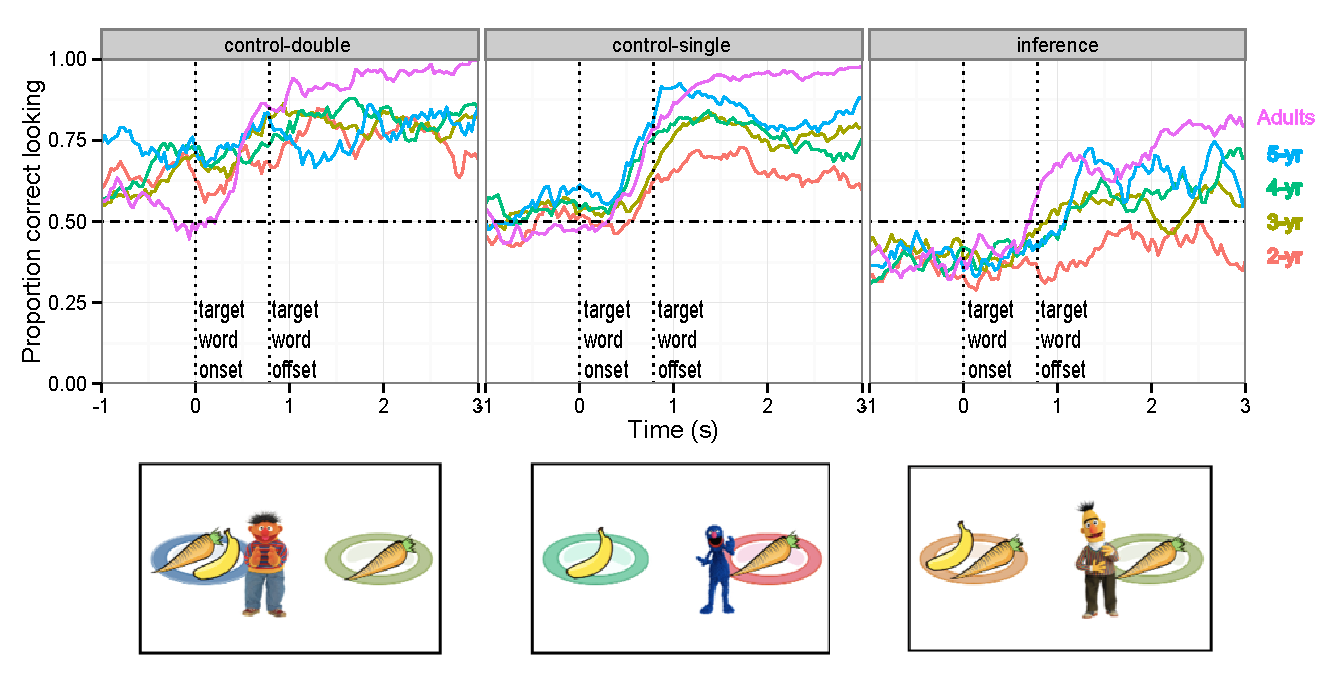
\includegraphics[width=.8\textwidth]{figures/expt1-accuracy.pdf}
  \caption{\label{fig:age} Proportion of 2- to 5-year-old children and adults looking to the target image as the utterance unfolds. Time 0 represents the target word onset. Proportion correct looking is defined by looks to the target divided by the total looks to both the target and the distractor. Bottom panels show example stimuli from each condition; the named character emerged at the end of the trial to mark the correct target.}
  \end{center} 
\end{figure*}


Participants of all ages looked to the targets in both control-double and control-single trials reliably above chance (50\%; Figure \ref{fig:age}). There were age differences in the speed of looking at the target and the proportion of correct looking across both control trial types, congruent with the findings of \citeA{fernald1998rapid}, who found that children's efficiency of familiar word recognition increases over the second year; the current data show this developmental pattern continuing throughout childhood. 

For inference trials, children of 4 years and above robustly looked to inferential targets (for 4-year-olds: $t(23) = 2.74$, $p =.01$). For example, upon hearing ``Bert's plate has a carrot,'' older children identified the plate with only a carrot as the referent rather than the plate with a carrot and a banana, replicating \citeA{stillerLLD}'s findings of ad-hoc implicature (though that study found successes in 3.5--4-year-old children as well). Although previous datasets are not directly comparable due to low-level differences in the task and materials, this finding is consistent with the hypothesis that children's inferential ability might have been obscured in previous SI tasks due to the unavailability of lexical alternatives (e.g. ``all'' given ``some''; \citeNP{huang2009semantic}).

One additional finding emerged: two-year-olds' looking at the target was below chance, rather than at chance: they tended to look more at distractors than targets ($t(23)  = 1.93$, $p = .066$) Hence, two-year-olds did not even seem to consider inferential targets and distractors as equally likely referents. Rather, they did not disengage from distractors relative to their baseline bias prior to hearing the target word. We return to this pattern and speculate about the sources for the developmental changes observed in the General Discussion. 

We fit a linear mixed-effects model \footnote{All mixed-effects models were run using the lme4 package in R Studio Version 0.98.932. The random effects structure for this model was as follows: (trial type $|$ subid) + (age $|$ item)} to measure the effects of trial type and age on the proportion of children looking to the target between 1 and 4s after noun onset (Table \ref{tab:lmer1}). We selected this time window because participants would have to wait until the end of target noun (0.8 seconds on average) to know they should switch to the inferential target, given the absence of a disambiguating continuation (e.g., ``Elmo's plate has a carrot \emph{and banana}.''). Results of the mixed-effects model indicate significant main effects of trial type and age: participants looked to the target significantly less in inference trials compared to control-single trials, and across all trial types, participants' looking to target increased with age. 

To look more closely at the effect of age within inference trials, we fit a linear mixed-effects model \footnote{The random effects structure for this model was as follows: (1 $|$ subid) + (age $|$ item)} to measure the effect of age on the proportion of children looking to the inferential target between the same time window (Table \ref{tab:lmer2}). Results indicate a significant main effect of age: participants looked toward the target at greater rates with increasing age.

\begin{table}[b!]
\caption{\label{tab:lmer1}  Coefficient estimates from mixed-effects models predicting proportion of looks to target in Experiment 1.} 
\begin{center} 
\begin{tabular}{l r r r l} 
\hline
Predictor  &  Value (SE) & \emph{t}-value\\
\hline
Intercept (Control-single)  & .60 (.05) & 12.30 \\
Age & .04 (.01) &  3.24 \\
Control-double & .10 (.06) & 1.81 \\
Inference & -.24 (.06) & -3.69 \\
Age $\times$ Control-double & -.02 (.01) & -1.14 \\
Age $\times$ Inference & .01 (.02) & .86 \\
\hline
\end{tabular} 
\end{center} 
\end{table}

We next analyzed participants' reaction times \cite{fernald2008looking}: We isolated trials on which participants were looking at the distractor at the point of disambiguation, and measured the average length of time prior to a shift to the target. Looks to the target were slower and overall lower in proportion in inference trials compared to both control trial types across all age groups (Figure \ref{fig:rt}). A linear mixed-effects model on trials on which participants were looking at the distractor at the point of disambiguation \footnote{The random effects structure for this model was as follows: (1 $|$ subid) + (age $|$ item)} indicated significant main effects of trial type and age on the average time before switch to targets: switch to the target was slower in inferential trials compared to control trials, and the amount of time before switch to the target decreased as age increased. Hence, implicatures were generally slower and harder to process compared to the unambiguous semantic meanings, regardless of the participants' age. 

\begin{figure}
\begin{centering} 
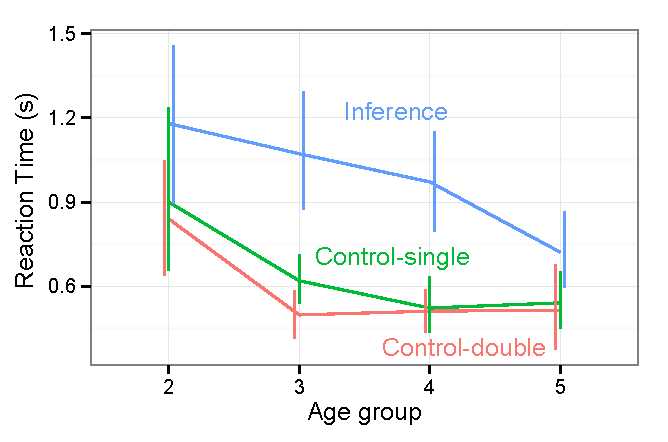
\includegraphics[width=3.2in]{figures/expt1-rt.pdf}
\caption{\label{fig:rt} Average reaction times for first switches to target in trials in which participants were looking at the distractor (and not the target) at the target word onset.}
\end{centering} 
\end{figure}

\section{Experiment 2}

\begin{table}[b!]
\caption{\label{tab:lmer2}  Coefficient estimates from mixed-effects models predicting proportion of looks to target in inference trials in Experiment 1.} 
\begin{center} 
\begin{tabular}{l r r r l} 
\hline
Predictor  &  Value (SE) & \emph{t}-value\\
\hline
Intercept  & .36 (.05) & 6.65 \\
Age & .06 (.01) &  3.96 \\
\hline
\end{tabular} 
\end{center} 
\end{table}

In Experiment 1, we found that children of 4 and above could compute implicatures given access to contextual alternatives. But children younger than 4 still struggled with implicature computation. In Experiment 2, we explored another factor that may improve children's performance: prosody. Contrastive stress---a change in pitch, characterized by an initial drop followed by a rise--- assists inference processing for both adults \cite{ito2008anticipatory} and preschool children \cite{kurumada1contextual}. For example, when preschoolers saw a picture of a zebra and a picture of an okapi that resembles a zebra, and heard ``It LOOKS like a zebra'' with a stress on the word ``look,'' they chose the picture of okapi if the context provided support. In the current experiment, we investigate whether a contrastive stress on the final noun (e.g., ``Elmo's plate has a CARROT'') in the inference trials would assist children in identifying the pragmatically-correct referent.

\subsection{Method}

\subsubsection{Participants}

Participants were recruited as in Experiment 1. For Experiment 2, we focused on 3- and 4-year-olds. Out of 57 initial participants, the final sample was chosen based on the same criteria as Experiment 1, and consisted of 17 3-year olds (8 girls), and 31 4-year olds (18 girls).

\subsubsection{Stimuli, Design, and Procedure}

The stimuli, design and procedure were identical to Experiment 1, except for one change: Target nouns in inference trials were produced with contrastive stress (low-high-low pitch accent and longer duration, 1.2 seconds on average). Based on previous findings that children identify contrastive prosody based on the norms set within an experiment \cite{kurumada1contextual}, we decided to include prosodic cues only in inference trials. 

\subsection{Results and Discussion}

\begin{figure*}[t]
	\center{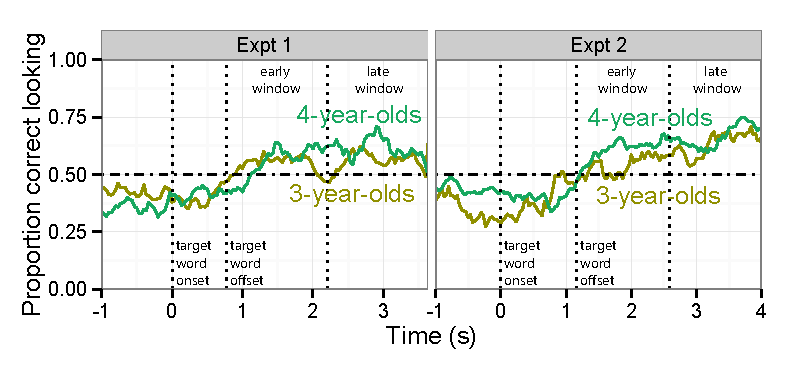
\includegraphics[width=.7\textwidth]{figures/expt2-accuracy.pdf}}
	\caption{\label{fig:pros0} Proportion of 3- and 4-year-old children looking to the target image as the utterance unfolds, comparing across two Experiments.}
\end{figure*}

To determine the effect of prosodic cues on children's inferential processing, we compared looking at targets across both Experiment 1 and 2 for inference trials (Figure \ref{fig:pros0}). Children's looking toward inferential targets increased slightly Experiment 2, especially towards the end of trials. In a post-hoc analysis, we split trials into an early and late period; Figure \ref{fig:0prosbar} shows this analysis directly. A linear mixed-effects model (Table \ref{tab:lmer3}) looking at the effects of age, trial type and window in Experiment 2 indicated a significant main effect of trial type, such that looking at target was lower in inference trials than in control trials. There was no significant interaction.

\begin{table}[b!]
\caption{\label{tab:lmer3}  Coefficient estimates from mixed-effects models predicting proportion of looks to target in Experiment 2.} 
\begin{center} 
\begin{tabular}{l r r r l} 
\hline
Predictor  &  Value (SE) & \emph{t}-value\\
\hline
Intercept (Control-single and Early)  & .80 (.04) & 21.04 \\
Age (4-year-old) & -.01 (.05) &  -.19 \\
Control-double & .03 (.05) & .59 \\
Inference & -.26 (.05) & -5.07 \\
Window (Late) & -.02 (.04) & -.46 \\
Age $\times$  Control-double & .04 (.06) & .65 \\
Age $\times$  Inference & .07 (.06) & 1.07 \\
Age $\times$  Window & .03 (.04) & .72 \\
Control-double $\times$  Window & .05 (.06) & .82 \\
Inference $\times$ Window & .10 (.06) & 1.73 \\
Age $\times$ Control-double $\times$ Window & -.07 (.07) & -.93 \\
Age $\times$ Inference $\times$ Window & -.03 (.07) & -.51 \\
\hline
\end{tabular} 
\end{center} 
\end{table}

A closer look at inference trials in the two Experiments suggested that 3-year-olds identified inferential targets when there were supportive prosodic cues. In Experiment 2, both 3- and 4-year-olds looked at the correct inferential target above chance (for 3-year-olds: $t(16) = 2.47$, $p < .03$; Figure \ref{fig:0prosbar}). This was in contrast to Experiment 1, in which 3-year-olds looked at the inferential target at chance level ($t(27) = 1.49$, $p = .15$). However, a linear mixed-effects model (Table \ref{tab:lmer4}) looking at the effects of experiment, age, and window in inference trials in Experiments 1 and 2 did not indicate an interaction between experiment and window. Based on these results, overall, 3-year-olds seem to be more successful when contextual alternatives and explicit stress both support implicature computation, in line with \citeA{stillerLLD}'s findings that 3.5-year-olds succeed in a similar behavioral implicature task. Nevertheless, the strength of contrastive stress as a cue for implicature computation is still uncertain, given the lack of a significant difference between the two Experiments. Looking at the effect of prosodic cue across more age groups or in a behavioral implicature task may help confirm its strength (see General Discussion for discussion on potential paradigmatic divergences). 

\section{General Discussion}

\begin{figure}[t]
\begin{center} 
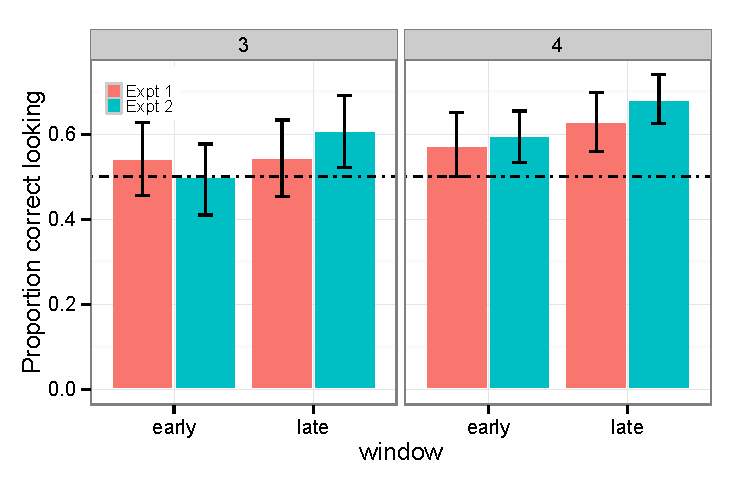
\includegraphics[width=3.2in]{figures/expt12-accuracy_inf.pdf}
\caption{\label{fig:0prosbar} Looking to the target as a proportion of looking to the target and distractor in inference trials, averaged during two time windows (early: first half of the window between offset and end of trial, late: second half of the window).}
\end{center} 
\end{figure}

\begin{table}[b!]
\caption{\label{tab:lmer4}  Coefficient estimates from mixed-effects models predicting proportion of looks to target in Inference trials in Experiment 1 and 2.} 
\begin{center} 
\begin{tabular}{l r r r l} 
\hline
Predictor  &  Value (SE) & \emph{t}-value\\
\hline
Intercept (Expt 1 and Early)  & .55 (.04) & 14.52 \\
Experiment (Expt 2)  & -.01 (.06) &  -.22 \\
Age (4-year-old) & -.01 (.05) &  -.23 \\
Window (Late) & .03 (.05) & .54 \\
Experiment $\times$  Age & .08 (.08) & 1.08 \\
Experiment $\times$  Window & .07 (.08) & .84 \\
Age $\times$  Window & .03 (.07) & .44 \\
Experiment $\times$ Age $\times$ Window & -.06 (.10) & -.60 \\
\hline
\end{tabular} 
\end{center} 
\end{table}

Are young children able to make online implicature inferences? The current work looked at children's processing of ad-hoc implicatures with an eye-tracking paradigm, and found that adults and children older than 3 years show robust looking toward the inferential targets, although at slower and overall lower rate compared to semantically unambiguous targets, whereas younger children still struggled with implicature computation. In Experiment 2, we found that prosodic cues with supportive context can help children as young as 3 to compute implicatures and identify inferential targets.

Our findings are broadly convergent with previous findings \cite{stillerLLD}, suggesting that the ability to make ad-hoc implicatures is fragile but measurable in 3-year-olds (with contrastive prosody) and more robust with 4-year-olds. Nevertheless, accuracy in the two paradigms differed: The rate of looking to the inferential target was overall lower in the current study than the accuracy rates in \citeA{stillerLLD}, even though the current paradigm was simpler (with two referent choices instead of three). This difference might be due to divergences between the two paradigms, since accuracy in our paradigm reflected graded patterns of looking rather than a single multi-alternative forced choice. 

One unpredicted and intriguing finding was that 2-year-olds not only did not look at the correct inferential target, but looked more toward the distractor. One potential explanation comes from the inhibitory demands of our task. The two potential referents in inference trials differed in saliency: The distractor was more salient as it contained an extra item (e.g., a carrot and a banana). Inhibitory control is difficult for children and continues to develop throughout the period we studied here (e.g.,  \citeNP{davidson2006development}). Congruent with this hypothesis, several recent studies suggest that inhibitory control might potentially affect word recognition in a number of similar eye-tracking paradigms \cite{yurovskybeyond,nordmeyer2013measuring}. Future work should thus address this possibility by explicitly manipulating the salience of potential pragmatic targets.

In sum, we found that preschool children were able to compute ad-hoc implicatures in contexts where there was substantial contextual support, in particular when they had access to lexical alternatives in the context, and when there were signals that emphasize the contrast between the target and its alternative. This is in line with previous claims that children's difficulties with SI are caused by their lack of access to linguistic scales (e.g., some-all; \citeNP{barner2011accessing}). 

The current work also sheds light on children's moment-to-moment processing of implicatures. It has previously been suggested that children are not able to compute SI's during online language comprehension (e.g., \citeNP{huang2009semantic}). The current work suggests another possibility: implicature computation may indeed be delayed compared to interpretations of unambiguous utterances, even for adults. However, with contextual access to scales relevant to implicature computation, children as young as 3 years could spontaneously generate implicature inferences. 

Even young children are sensitive to the communicative intentions behind utterances they hear \cite{clark2009first,baldwin1993early}. Our work adds to the body of evidence suggesting that by preschool age they generate sophisticated pragmatic implicatures as well, even though these inferences are easily masked by other processing demands of specific contexts and situations. Overall, our current work takes one step further towards reconciling children's early-emerging communicative abilities with the complex pattern of successes and failures that they show in Gricean pragmatics.

\section{Acknowledgments}

We thank the parents, children, and staff at the San Jose Children's Discovery Museum. This work was supported by a Postgraduate Scholarship and Doctoral Program Fellowship provided by Natural Sciences and Engineering Research Council of Canada.

\bibliographystyle{apacite}

\setlength{\bibleftmargin}{.125in}
\setlength{\bibindent}{-\bibleftmargin}

\bibliography{YoonCogSci15}


\end{document}
